\section{Least Angle Regression}
\begin{frame}
    \frametitle{Least Angle Regression}
\begin{enumerate}
    \item Forward Stepwise Selection
    \item Forward Stagewise Selection
    \item Least Angle Regression
\end{enumerate}
\end{frame}

\begin{frame}
\frametitle{Forward Stepwise Selection}
A simple example in the case of $p=2$ predictors.

\begin{columns}[t]
    \column{0.5\textwidth}
    \begin{enumerate}
        \item Start with a null model.
    \end{enumerate}
    
    \column{0.5\textwidth}
    \begin{figure}[!htbp]
        \begin{center}
            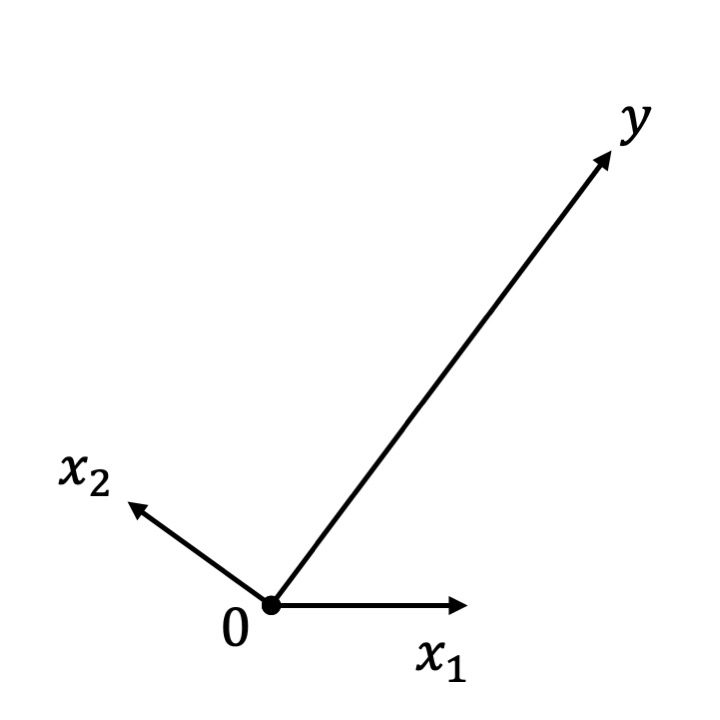
\includegraphics[width=0.9\textwidth]{img/FStepR/1.jpeg}
        \end{center}
    \end{figure}
\end{columns}
\end{frame}

\begin{frame}
\frametitle{Forward Stepwise Selection}
A simple example in the case of $p=2$ predictors.

\begin{columns}[t]
    \column{0.5\textwidth}
    \begin{enumerate}
        \item Start with a null model.
        \item Find the predictor most correlated with the response and perform simple linear regression.
    \end{enumerate}
    
    \column{0.5\textwidth}
    \begin{figure}[!htbp]
        \begin{center}
            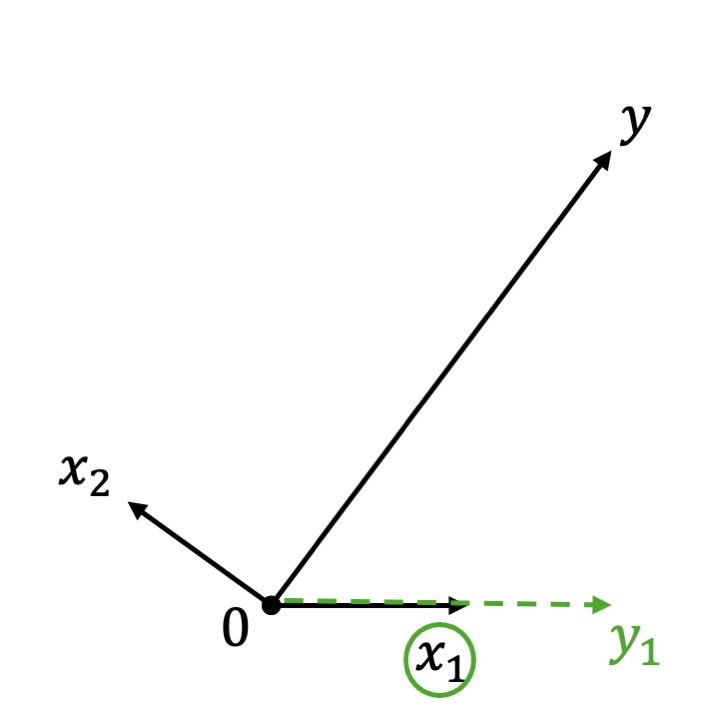
\includegraphics[width=0.9\textwidth]{img/FStepR/2.jpeg}
        \end{center}
        % \caption{Regression with Forward Stepwise Selection}
    \end{figure}
    \end{columns}
\end{frame}

\begin{frame}
\frametitle{Forward Stepwise Selection}
A simple example in the case of $p=2$ predictors.

\begin{columns}[t]
    \column{0.5\textwidth}
    \begin{enumerate}
        \item Start with a null model.
        \item Find the predictor most correlated with the response and perform simple linear regression.
        \item Set the residuals as the new response.
    \end{enumerate}
    
    \column{0.5\textwidth}
    \begin{figure}[!htbp]
        \begin{center}
            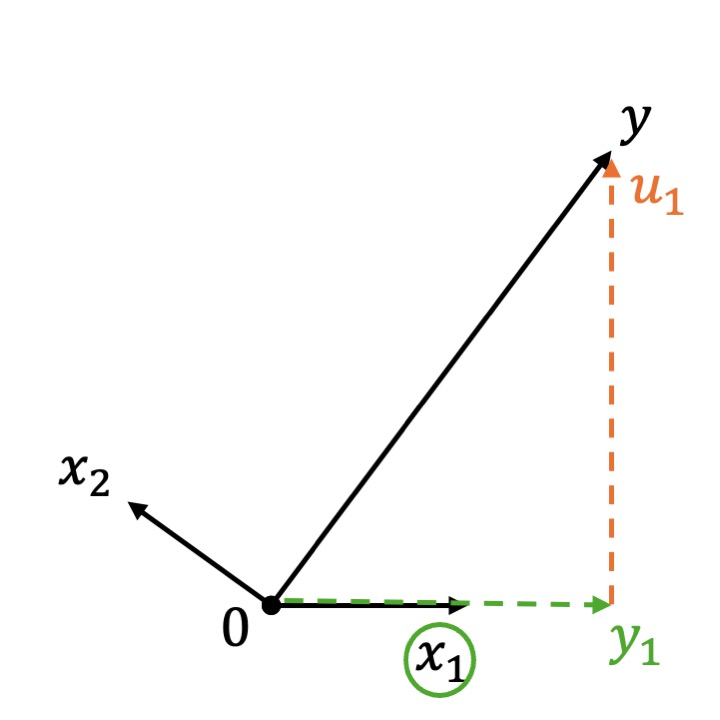
\includegraphics[width=0.9\textwidth]{img/FStepR/3.jpeg}
        \end{center}
        % \caption{Regression with Forward Stepwise Selection}
    \end{figure}
    \end{columns}
\end{frame}

\begin{frame}
\frametitle{Forward Stepwise Selection}
A simple example in the case of $p=2$ predictors.

\begin{columns}[t]
    \column{0.5\textwidth}
    \begin{enumerate}
        \item Start with a null model.
        \item Find the predictor most correlated with the response and perform simple linear regression.
        \item Set the residuals as the new response.
        \item Project other predictors orthogonal to the predictor selected in previous step.
    \end{enumerate}
    
    \column{0.5\textwidth}
    \begin{figure}[!htbp]
        \begin{center}
            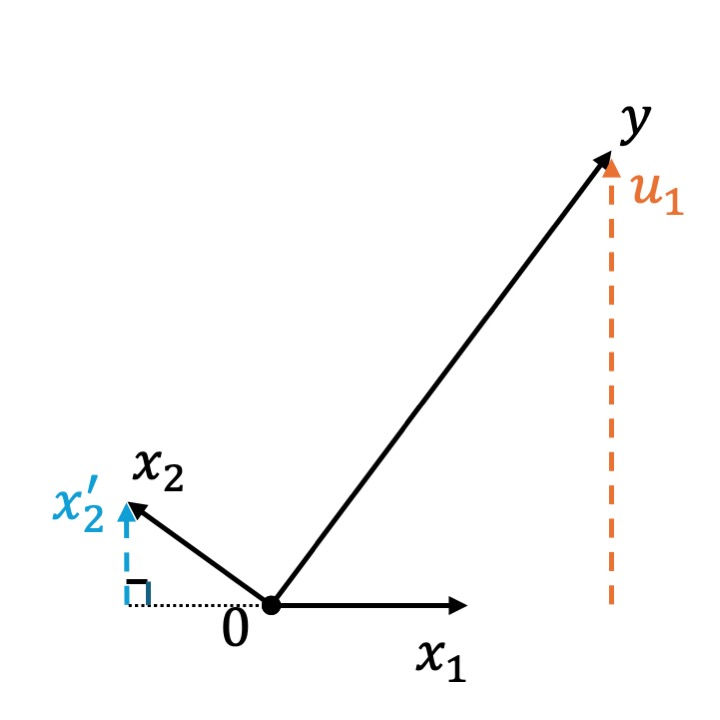
\includegraphics[width=0.9\textwidth]{img/FStepR/4.jpeg}
        \end{center}
        % \caption{Regression with Forward Stepwise Selection}
    \end{figure}
    \end{columns}
\end{frame}

\begin{frame}
\frametitle{Forward Stepwise Selection}
A simple example in the case of $p=2$ predictors.

\begin{columns}[t]
    \column{0.5\textwidth}
    \begin{enumerate}
        \item Start with a null model.
        \item Find the predictor most correlated with the response and perform simple linear regression.
        \item Set the residuals as the new response.
        \item Project other predictors orthogonal to the predictor selected in previous step.
        \item Repeat steps $2-4$ until the stopping criterion is met.
    \end{enumerate}
    
    \column{0.5\textwidth}
    \begin{figure}[!htbp]
        \begin{center}
            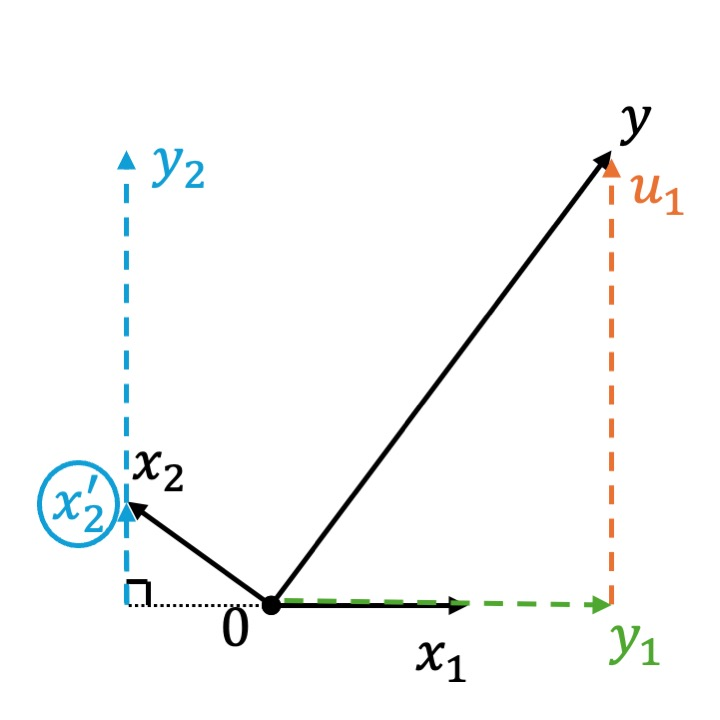
\includegraphics[width=0.9\textwidth]{img/FStepR/5.jpeg}
        \end{center}
        % \caption{Regression with Forward Stepwise Selection}
    \end{figure}
    \end{columns}
\end{frame}

%---------------------------------------------------------
\begin{frame}
\frametitle{Forward Stagewise Selection}
In contrast to forward stepwise selection, forward stagewise selection builds the model in successive small steps $\varepsilon$.

\begin{columns}[t]
    \column{0.5\textwidth}
    Let $\hat{\mathbf{\mu}}$ be the current Stagewise estimate and $\hat{\mathbf{c}}=\mathbf{c}(\hat{\mathbf{\mu}})=X^T(y-\hat{\mathbf{\mu}})$ be the vector of current correlations. Therefore, $\hat{c}_j$ is proportional to the correlation between the covariate $x_j$ and the current residual vector.
    \begin{enumerate}
        \item Start with $\hat{\mathbf{\mu}}=0$ and a null model.
    \end{enumerate}
    
    \column{0.5\textwidth}
    \begin{figure}[!htbp]
        \begin{center}
            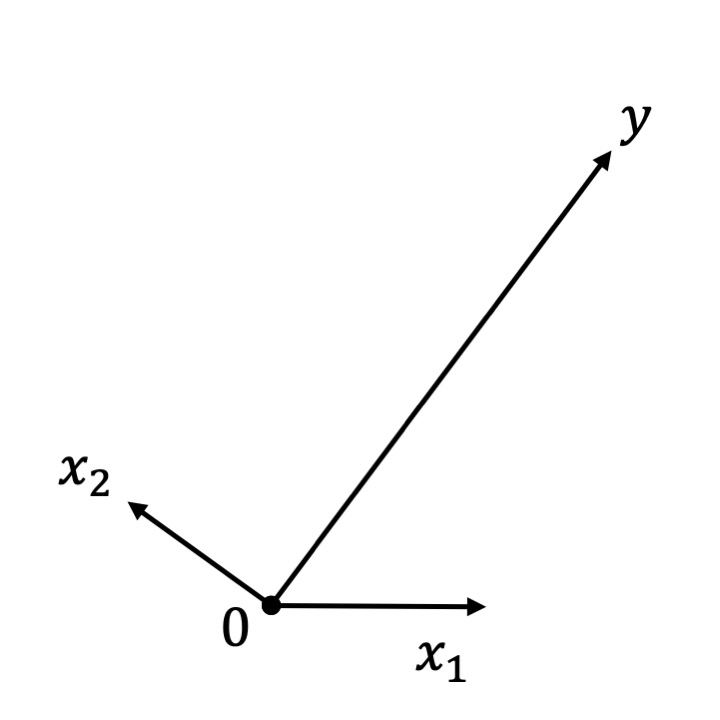
\includegraphics[width=0.9\textwidth]{img/FStageR/1.jpeg}
        \end{center}
    \end{figure}
\end{columns}
\end{frame}

\begin{frame}
\frametitle{Forward Stagewise Selection}
Let $\hat{\mathbf{\mu}}$ be the current Stagewise estimate and $\hat{\mathbf{c}}=\mathbf{c}(\hat{\mathbf{\mu}})=X^T(y-\hat{\mathbf{\mu}})$ be the vector of current correlations.

\begin{columns}[t]
    \column{0.5\textwidth}
    \begin{enumerate}
        \item Start with $\hat{\mathbf{\mu}}=0$ and a null model.
        \item Find the predictor $j$ that has the highest correlation that $\hat{j}=\arg\max_{j}|\hat{c}_j|$.
        \item Update $\hat{\mathbf{\mu}}\leftarrow\hat{\mathbf{\mu}}+\varepsilon\cdot\text{sign}(\hat{c}_{\hat{j}})\cdot\mathbf{x}_{\hat{j}}$ and $\mathbf{\hat{c}}$.
        \item Repeat steps $2-3$ until the stopping criterion is met.
    \end{enumerate}
    
    \column{0.5\textwidth}
    \begin{figure}[!htbp]
        \begin{center}
            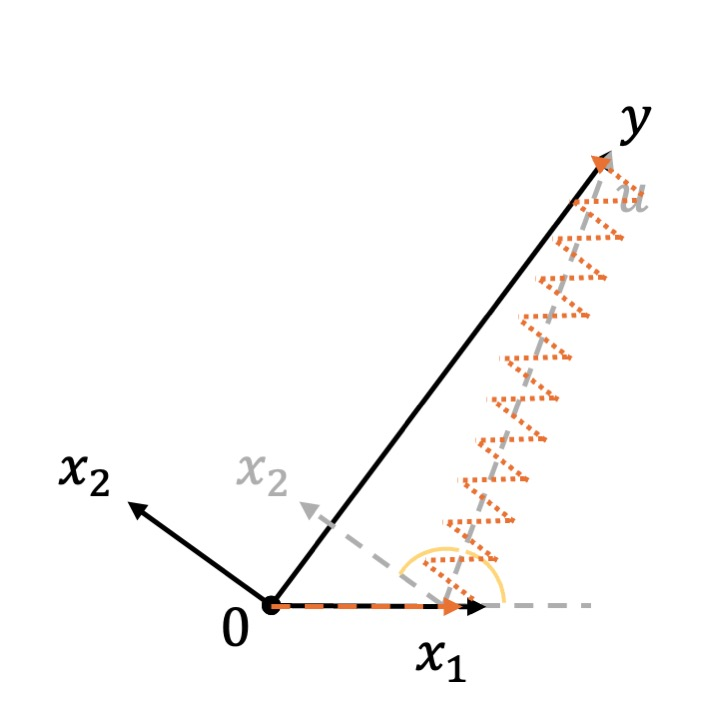
\includegraphics[width=0.9\textwidth]{img/FStageR/2.jpeg}
        \end{center}
    \end{figure}
\end{columns}
\end{frame}

%---------------------------------------------------------
\begin{frame}
\frametitle{Least Angle Regression: Example}
Least Angle Regression (LAR) is a stylized version of forward stagewise procedure that uses a simple mathematical formula to accelerate the computations.

\begin{columns}[t]
    \column{0.5\textwidth}
    \begin{enumerate}
        \item Start with $\hat{\mathbf{\mu}}=0$ and a null model.
    \end{enumerate}
    
    \column{0.5\textwidth}
    \begin{figure}[!htbp]
        \begin{center}
            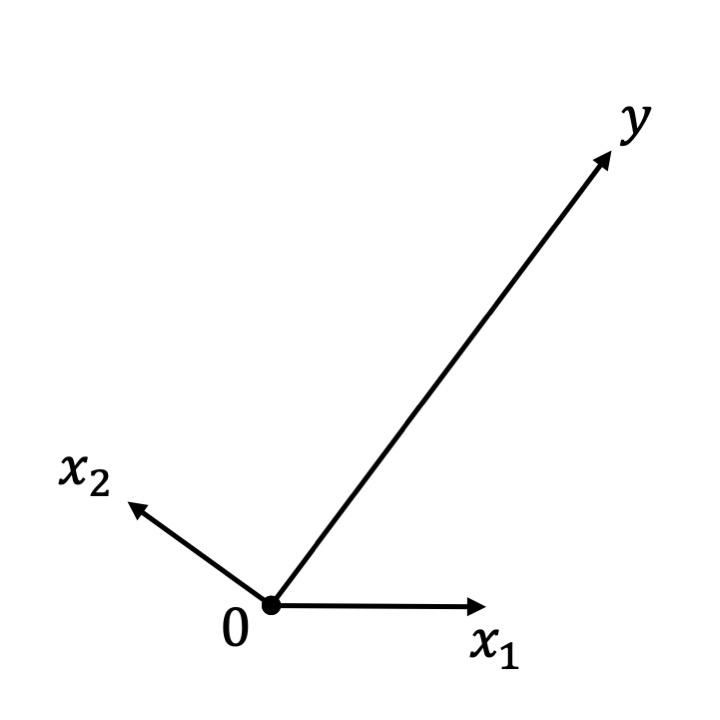
\includegraphics[width=0.9\textwidth]{img/LAR/1.jpeg}
        \end{center}
    \end{figure}
\end{columns}
\end{frame}

\begin{frame}
\frametitle{Least Angle Regression: Example}
\begin{columns}[t]
    \column{0.5\textwidth}
    \begin{enumerate}
        \item Start with $\hat{\mathbf{\mu}}=0$ and a null model.
        \item Find the predictor most correlated with the response.
    \end{enumerate}
    
    \column{0.5\textwidth}
    \begin{figure}[!htbp]
        \begin{center}
            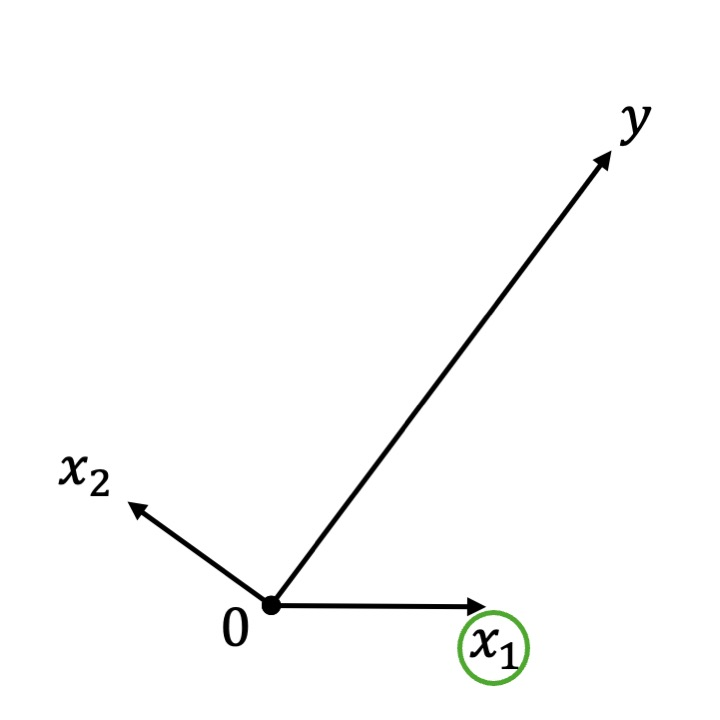
\includegraphics[width=0.9\textwidth]{img/LAR/2.jpeg}
        \end{center}
    \end{figure}
\end{columns}
\end{frame}

\begin{frame}
\frametitle{Least Angle Regression: Example}
\begin{columns}[t]
    \column{0.5\textwidth}
    \begin{enumerate}
        \item Start with $\hat{\mathbf{\mu}}=0$ and a null model.
        \item Find the predictor most correlated with the response.
        \item Take the largest step possible in the direction of this predictor until some other predictor has as much correlation with the current residual.
    \end{enumerate}
    
    \column{0.5\textwidth}
    \begin{figure}[!htbp]
        \begin{center}
            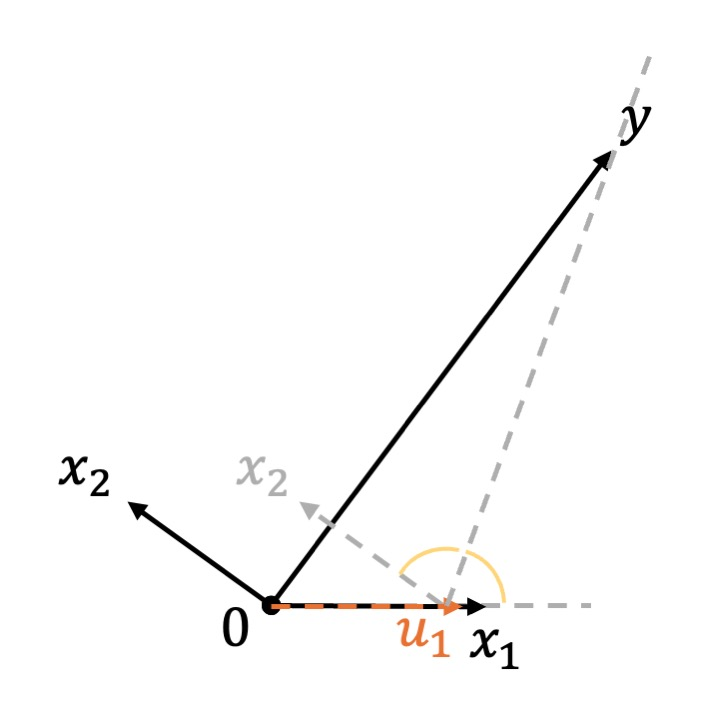
\includegraphics[width=0.9\textwidth]{img/LAR/3.jpeg}
        \end{center}
    \end{figure}
\end{columns}
\end{frame}

\begin{frame}
\frametitle{Least Angle Regression: Example}
\begin{columns}[t]
    \column{0.6\textwidth}
    \begin{enumerate}
        \item Start with $\hat{\mathbf{\mu}}=0$ and a null model.
        \item Find the predictor most correlated with the response.
        \item Take the largest step possible in the direction of this predictor until some other predictor has as much correlation with the current residual.
        \item The new direction is the equiangular vector of the two predictors. Move in until a third predictor earns its way into the ``most correlated'' set.
        \item Repeat steps $3-4$ until met the stopping criterion.
    \end{enumerate}
    
    \column{0.5\textwidth}
    \begin{figure}[!htbp]
        \begin{center}
            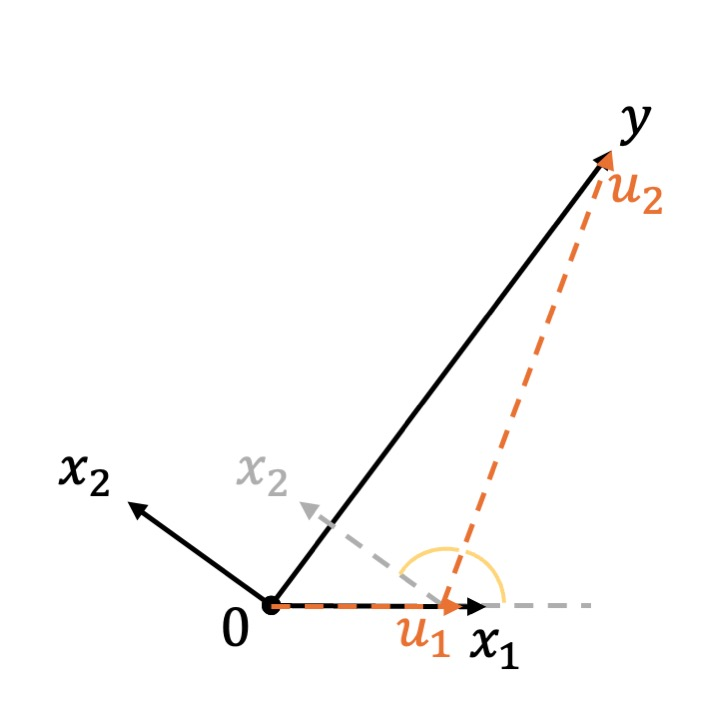
\includegraphics[width=0.9\textwidth]{img/LAR/4.jpeg}
        \end{center}
    \end{figure}
\end{columns}
\end{frame}

\begin{frame}
    \frametitle{Least Angle Regression: L1 Arc Length}
\begin{figure}[!htbp]
    \begin{center}
        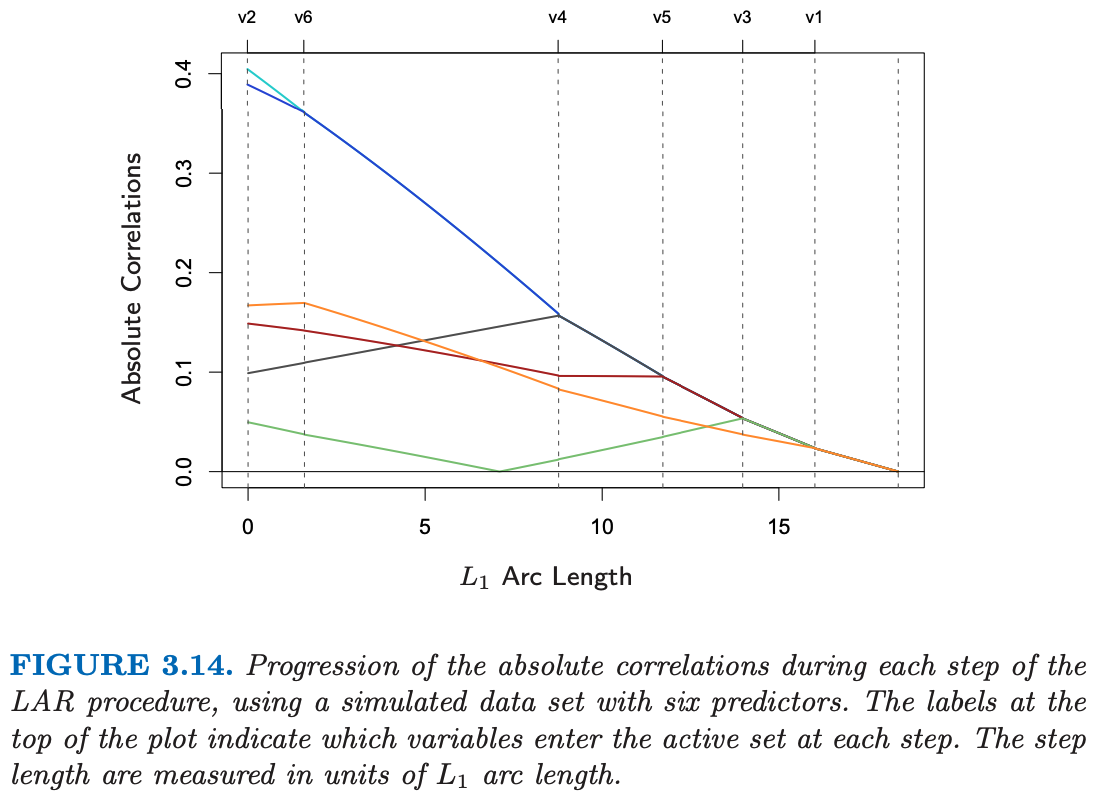
\includegraphics[width=0.8\textwidth]{img/L1ArcLength.png}
    \end{center}
    % \caption{}\label{fig:}
\end{figure}
\end{frame}

\begin{frame}
\frametitle{Least Angle Regression: The Equiangular Vector}
Assume that $\mathbf{x}_1,\dots,\mathbf{x}_p$ are linearly independent and for $\mathcal{A}$ a subset of indices $\{1,\dots,p\}$, define the matrix $\mathbf{X}_\mathcal{A}={(\dots,s_j\mathbf{x}_j,\dots)}_{j\in\mathcal{A}}$ where signs $s_j$ equal $\pm 1$. Let
\begin{equation}
    g_\mathcal{A}=\mathbf{X}_\mathcal{A}^T\mathbf{X}_\mathcal{A}
    \quad \text{and} \quad
    A_\mathcal{A}={(\mathbf{1}^T_\mathcal{A}g^{-1}_\mathcal{A}\mathbf{1}_\mathcal{A})}^{-1/2},\label{eq:lars25}
\end{equation}
where $\mathbf{1}_\mathcal{A}$ is a vector of ones of length $|\mathcal{A}|$. The equiangular vector $\mathbf{u}_\mathcal{A}$ is defined as
\begin{equation}
    \mathbf{u}_\mathcal{A}=\mathbf{X}_\mathcal{A}\omega_\mathcal{A}, \text{ where } \omega_\mathcal{A}=A_\mathcal{A} g^{-1}_\mathcal{A}\mathbf{1}_\mathcal{A},\label{eq:lars26}
\end{equation}
is the unit vector making equal angles, less than $90^\circ$, with the columns of $\mathbf{X}_\mathcal{A}$ satisfying $\mathbf{X}_\mathcal{A}^T\mathbf{u}_\mathcal{A}=A_\mathcal{A}\mathbf{1}_\mathcal{A}$ and $\|\mathbf{u}_\mathcal{A}\|=1$.
\end{frame}

\begin{frame}
\frametitle{Least Angle Regression: Algorithm}
% Then the algorithm of LARS comes as follows:
\begin{enumerate}
    \item Initialize all the coefficients $\hat{\mathbf{\mu}}_0$ as 0, and let the residual $\mathbf{u}=\mathbf{y}$.
    \item Suppose that $\hat{\mathbf{\mu}}_\mathcal{A}$ is the current estimate of coefficients and $\hat{\mathbf{c}}=\mathbf{c}(\hat{\mathbf{\mu}}_\mathcal{A})=X^T(y-\hat{\mathbf{\mu}}_\mathcal{A})$ are the current correlations. The active set $\mathcal{A}$ is the set of indices corresponding to covariates with the greatest absolute correlations, i.e., $\mathcal{A}=\{j:|\hat{c}_j|=\hat{\mathbf{C}}\}$ and $\hat{\mathbf{C}}=\max_{j}|\hat{c}_j|$.
    
    Let $s_j=\text{sign}(\hat{c}_j)$ for $j\in\mathcal{A}$, and compute $A_\mathcal{A}$, and $\mathbf{u}_\mathcal{A}$ as in (\ref{eq:lars25}) and (\ref{eq:lars26}). Also, compute the inner product $\mathbf{a}=:X^T\mathbf{u}_\mathcal{A}$. Updates $\hat{\mathbf{\mu}}_\mathcal{A}$ as
    \begin{equation}\label{eq:lars212}
        \hat{\mathbf{\mu}}_\mathcal{A}\leftarrow\hat{\mathbf{\mu}}_\mathcal{A}+\hat{\gamma}\mathbf{u}_\mathcal{A},
    \end{equation}
    where $\hat{\gamma}=\min_{j\in\mathcal{A}^c}^+\left(\frac{\hat{\mathbf{C}}-\hat{c}_j}{A_\mathcal{A}-\mathbf{a}_j}, \frac{\hat{\mathbf{C}}+\hat{c}_j}{A_\mathcal{A}+\mathbf{a}_j}\right)$; ``$\min^+$'' denotes the minimum taken over only positive quantities.
    \item Repeat step 2 until the stopping criterion is met.
\end{enumerate}
    
\end{frame}

%---------------------------------------------------------
\begin{frame}
\frametitle{Extend LAR to Lasso Regression}
If a non-zero coefficient hits zero, drop its variable from the active set and recompute the current joint least squares direction. This is the modification to LAR for Lasso.

Define $\hat{\mathbf{d}}$ to be the $m$-vector equaling $s_j{ \{A_\mathcal{A} g^{-1}_\mathcal{A} \mathbf{1}_\mathcal{A}\}}_j$ for $j\in\mathcal{A}$ and zero elsewhere. 

Let $$\tilde{\gamma}=\min_{\gamma_j>0}\{\gamma_j\},$$ where $\gamma_j=-\hat{\beta}_j/\hat{d}_j$, we have the following modification to LAR for Lasso:

\begin{block}{LASSO MODIFICATION}
If $\tilde{\gamma}<\hat{\gamma}$, stop the ongoing LARS at $\gamma=\tilde{\gamma}$ and remove $\tilde{j}$ from the active set. Then continue the LARS path from the current point.
\end{block}
\end{frame}

\begin{frame}
\frametitle{Extend LAR to Stagewise Regression}
If we modify the active set $\mathcal{A}$ (so that $\omega_\mathcal{A}$ would not have negative components), we can extend LAR to Stagewise Regression.

Define
$$P\equiv(N_1,\dots,N_p)/N, \quad \mathcal{C}_{\mathcal{A}}=\left\{\mathbf{v}=\sum_{j\in\mathcal{A}}s_j \mathbf{x}_j P_j, P_j\geq 0\right\}$$ 
where $N_j\equiv \#\{\text{steps with selected index j}\}$. Then we have the following modification to LAR for Stagewise Regression:

\begin{block}{STAGEWISE MODIFICATION}
Replace the $\mathbf{u}_{\mathcal{A}}$ in LAR with $\mathbf{u}_{\hat{\mathcal{B}}}$, the unit vector lying alone the projection of $\mathbf{u}_{\mathcal{A}}$ into $\mathcal{C}_{\mathcal{A}}$.
\end{block}
\end{frame}

\begin{frame}
    \frametitle{Comparison the Solution Paths of LARS}
\begin{figure}[!htbp]
    \begin{center}
        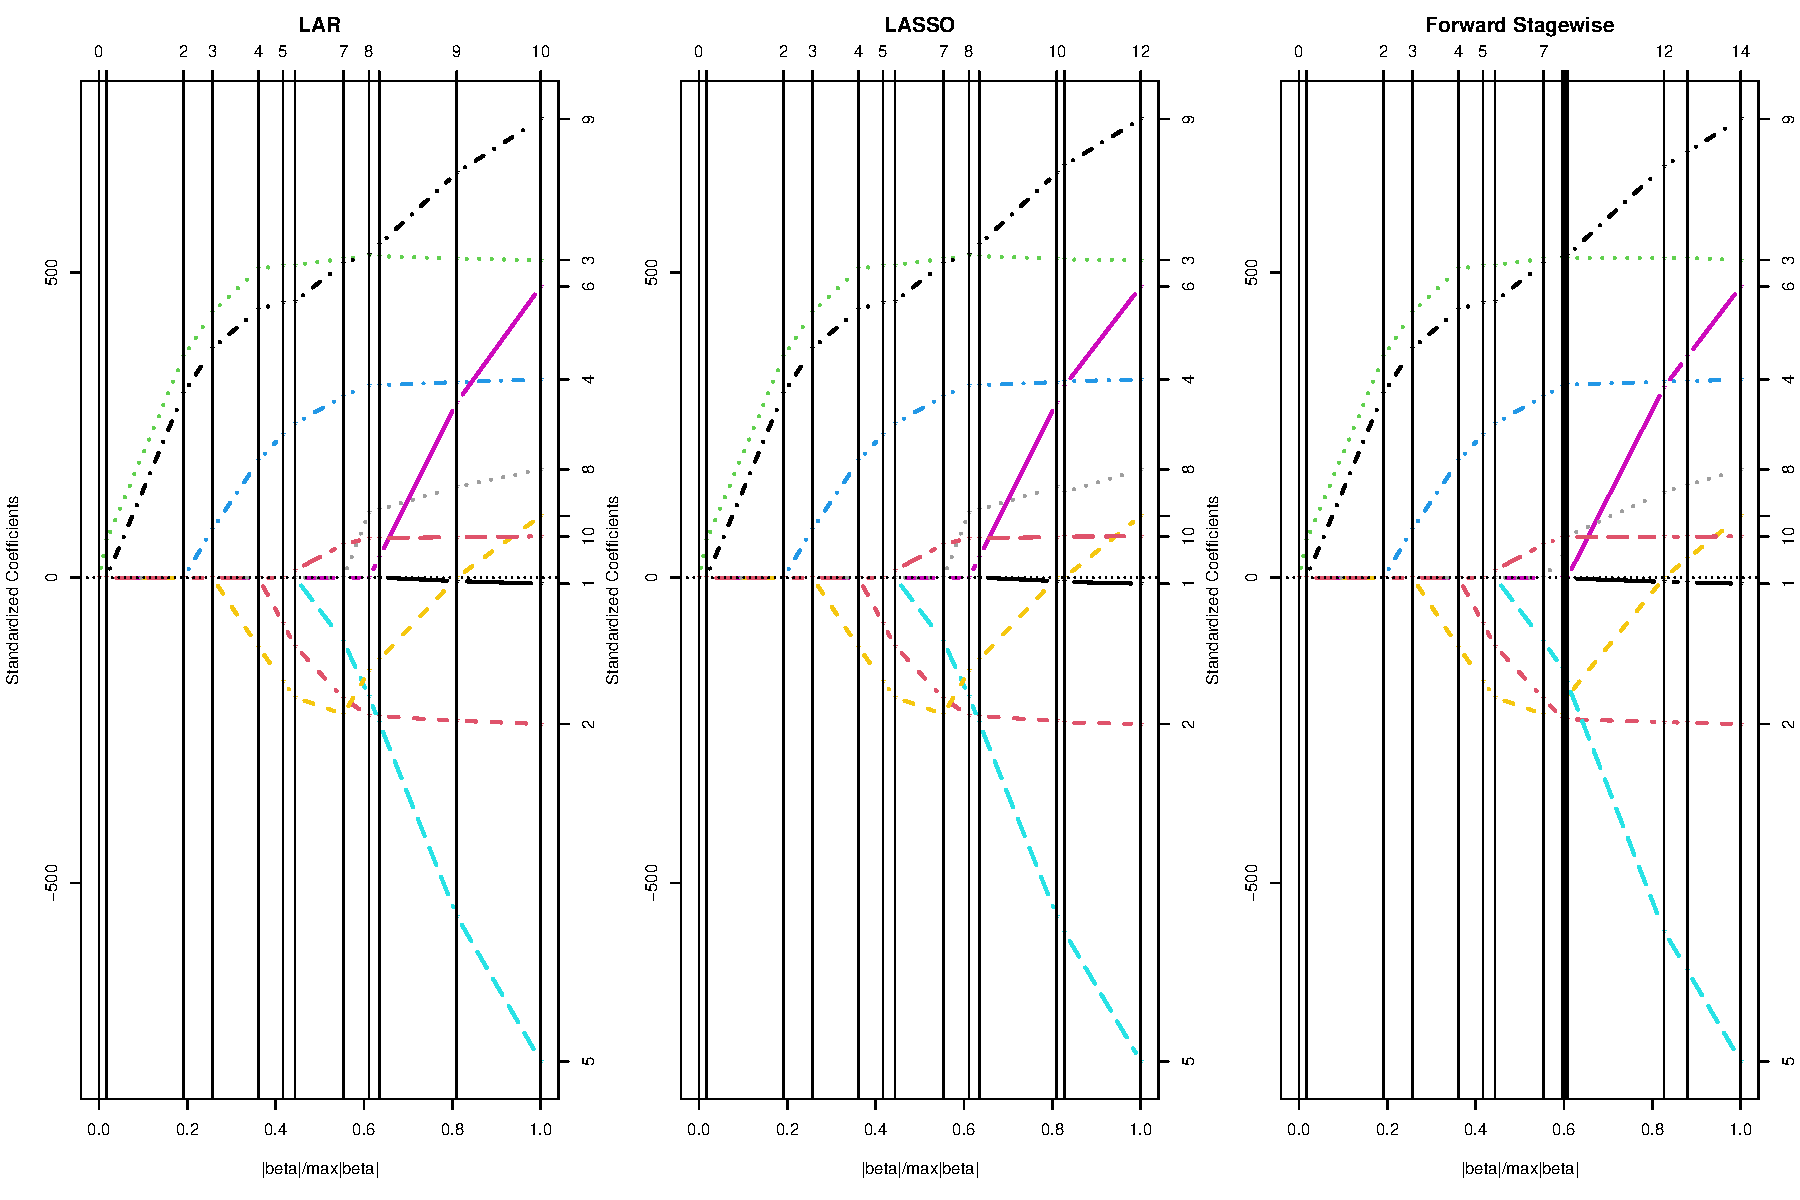
\includegraphics[width=0.75\textwidth]{img/lars_diabetes.pdf}
    \end{center}
    \caption{Solution paths of LAR, LAR-lasso and Forward Stagewise Selection for the diabetes data set.}\label{fig:lars_diabetes}
\end{figure}
\end{frame}

\begin{frame}
    \frametitle{Comparison of Computational Time}
\begin{figure}[!htbp]
    \begin{center}
        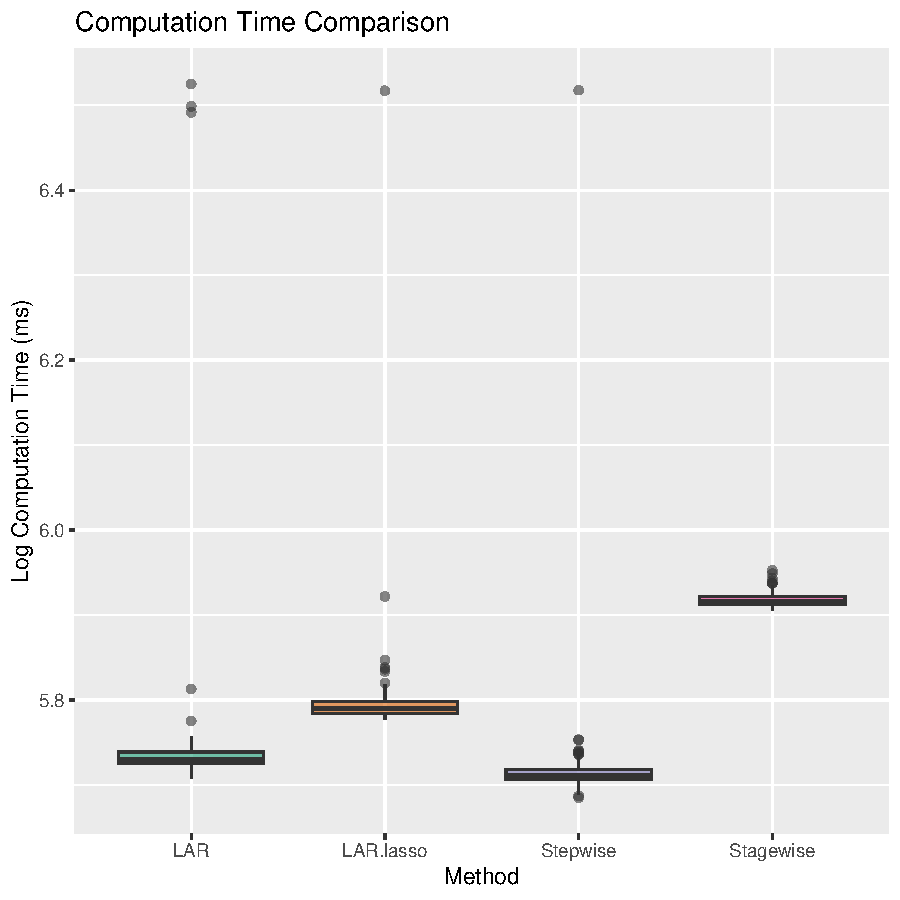
\includegraphics[width=0.5\textwidth]{img/lars_time.pdf}
    \end{center}
    \caption{Comparison of computational time between LAR, LAR-Lasso, Forward Stagewise Selection, and Forward Stepwise Selection with the diabetes data set.}\label{fig:lars_time}
\end{figure}
\end{frame}

%---------------------------------------------------------
\section{Coordinate Descent}
\begin{frame}
    \frametitle{Coordinate Descent: Motivation Question 1}
To motivate the objective function we would like to deal with using coordinate descent, let's consider these questions first:

Q1: Does $f\left(x+\delta e_i\right) \geq f(x)$ for all $\delta, i \Rightarrow f(x)=\min _z f(z)$ (Here $e_i=(0, \ldots, 1, \ldots 0)$, the $i$-th standard basis vector) always hold?

In other words, given convex, differentiable $f: R^n \rightarrow R$, if we are at a point $x$ such that $f(x)$ is minimized along each coordinate axis, then have we found a global minimizer?
\end{frame}

\begin{frame}
    \frametitle{Coordinate Descent: Motivation Question 1}
Q1: Does $f\left(x+\delta e_i\right) \geq f(x)$ for all $\delta, i \Rightarrow f(x)=\min _z f(z)$ (Here $e_i=(0, \ldots, 1, \ldots 0)$, the $i$-th standard basis vector) always hold?

Yes. $\textbf{Proof}$:
$$
f\left(x+\delta e_i\right) \geq f(x) \Rightarrow \frac{\partial f}{\partial x_i}(x)=0,
$$
which means
$$
\nabla f(x)=\left(\frac{\partial f}{\partial x_1}(x), \ldots, \frac{\partial f}{\partial x_n}(x)\right)=0
$$

Then we get $f(x)=\min_z f(z)$.
\end{frame}

\begin{frame}
    \frametitle{Coordinate Descent: Motivation Question 2}
Q2: Same question, but $f$ is convex, not differentiable?
\pause
\begin{figure}[!htbp]
    \begin{center}
        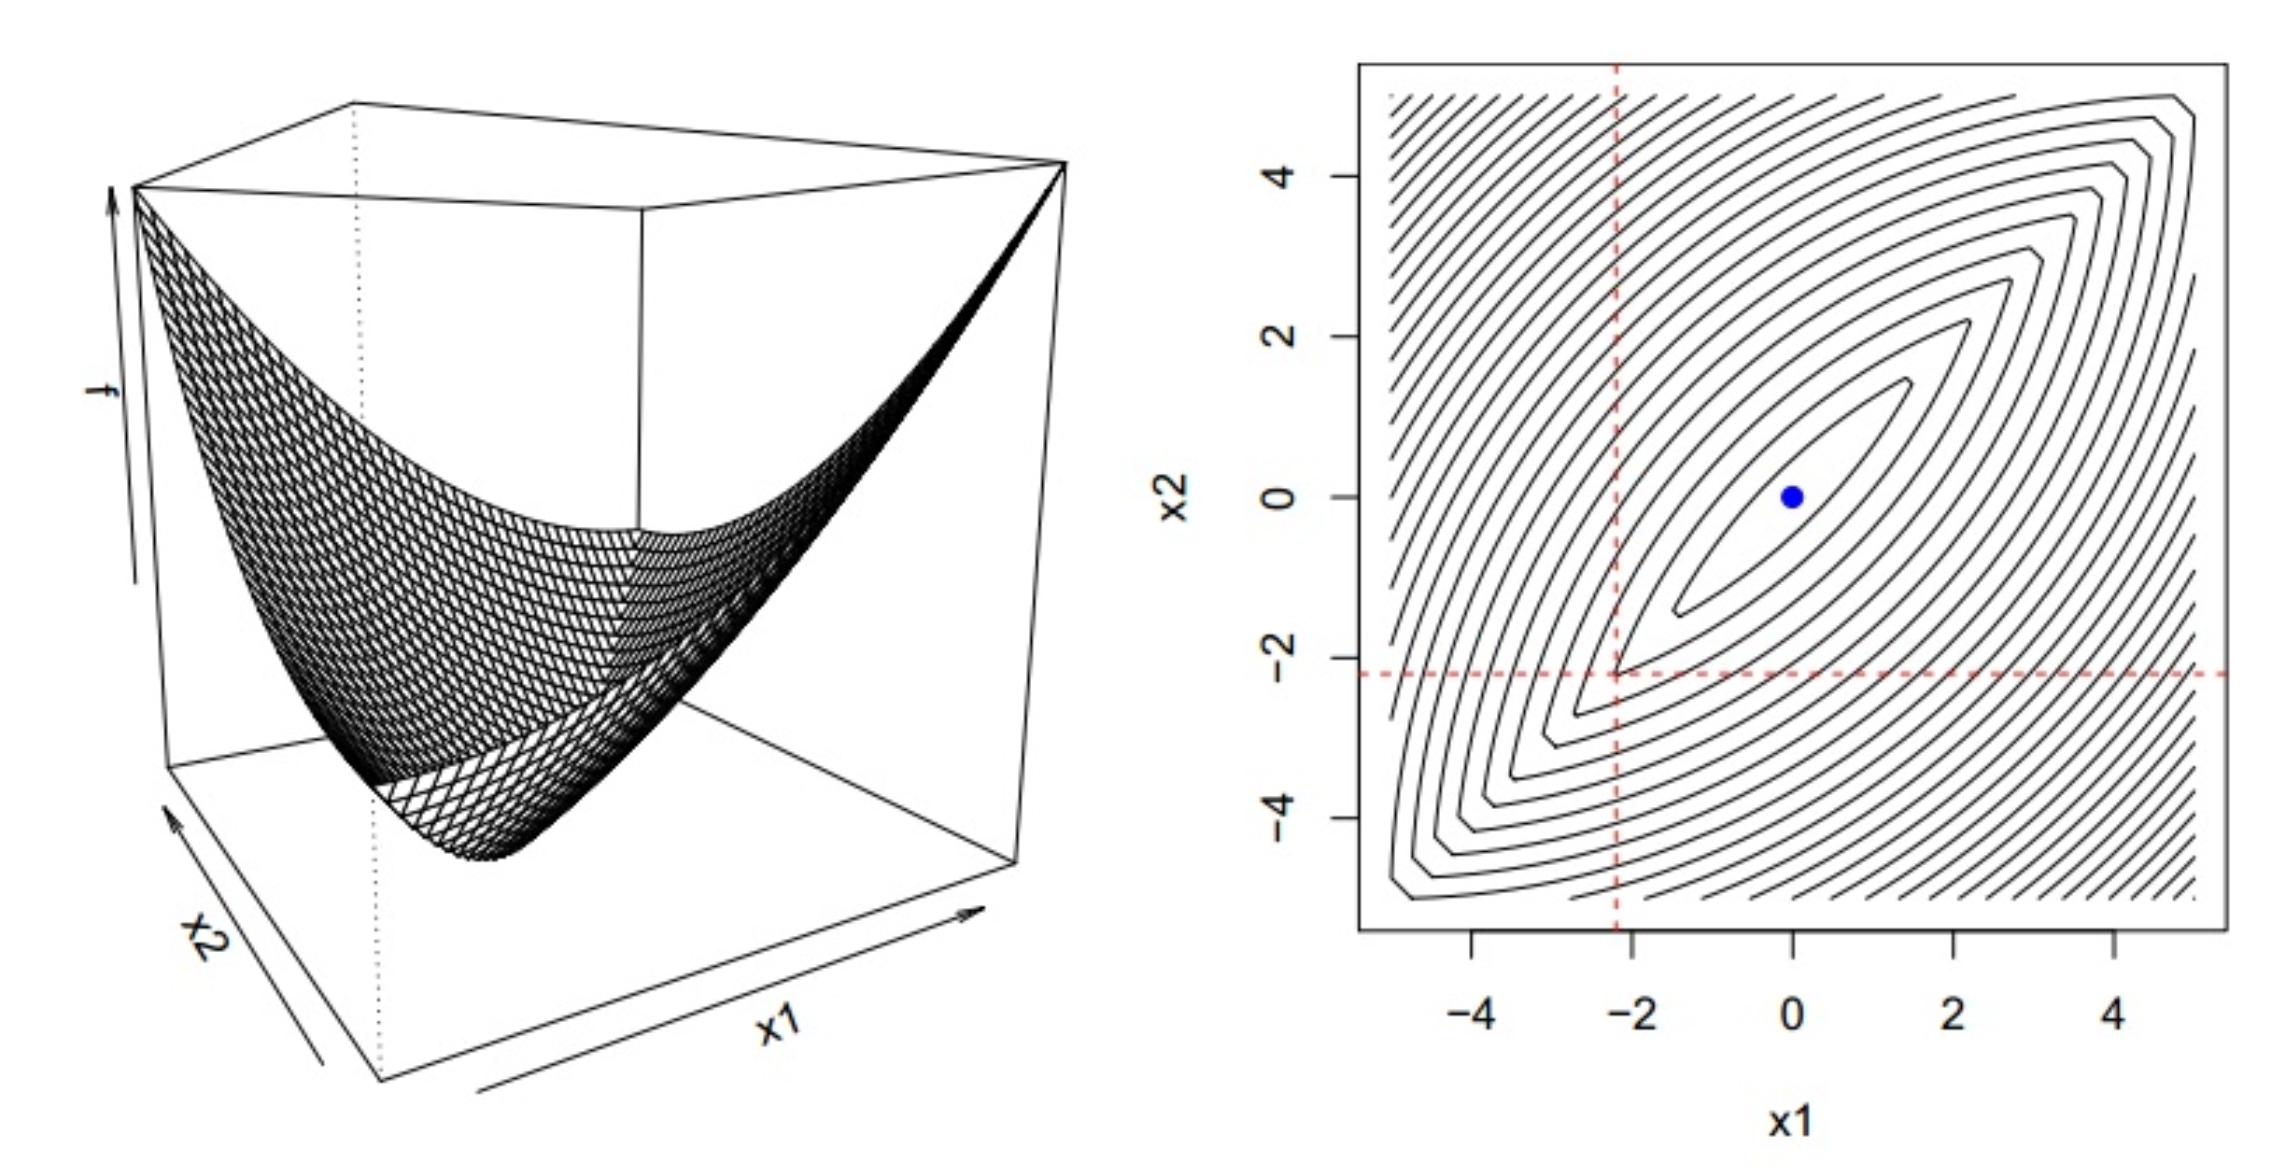
\includegraphics[width=0.6\textwidth]{img/cd_q2.png}
    \end{center}
    \caption{$f$ is not differentiable along the diagonal, but is convex. The global minimizer is at the origin (centre).}\label{fig:cd_q2}
\end{figure}

No. We can see that the cross-point is minimized for each axis, but only the origin is the global minimizer.
\end{frame}

\begin{frame}
\frametitle{Coordinate Descent: Motivation Question 3}
Q3: Same question again, but now $f(x)=g(x)+\sum_{i=1}^n h_i\left(x_i\right)$, where $g(x)$ is convex, differentiable and each $h_i$ is just convex (Here the non-smooth part is called separable)?
\end{frame}

\begin{frame}
\frametitle{Coordinate Descent: Motivation Question 3}
Q3: Same question again, but now $f(x)=g(x)+\sum_{i=1}^n h_i\left(x_i\right)$, where $g(x)$ is convex, differentiable and each $h_i$ is just convex?

Yes. $\textbf{Proof}$: Since $g(x)$ is convex, differentiable, for any $y$, we have
\begin{align*}
    f(y)-f(x)&=g(y)+\sum_{i=1}^n h_i\left(y_i\right)-\left[g(x)+\sum_{i=1}^n h_i\left(x_i\right)\right] \\
    &\geq \nabla g(x)^T(y-x)+\sum_{i=1}^n\left[h_i\left(y_i\right)-h_i\left(x_i\right)\right]\\
    &=\sum_{i=1}^n\left(\nabla_i g(x)\left(y_i-x_i\right)+h_i\left(y_i\right)-h_i\left(x_i\right)\right)
\end{align*}

We now want to proof
\begin{equation}
    \nabla_i g(x)\left(y_i-x_i\right)+h_i\left(y_i\right)-h_i\left(x_i\right) \geq 0.
\end{equation}
\end{frame}

\begin{frame}
\frametitle{Coordinate Descent: Motivation Question 3}
We now want to proof
$$\nabla_i g(x)\left(y_i-x_i\right)+h_i\left(y_i\right)-h_i\left(x_i\right) \geq 0.$$
Consider $f_i\left(x_i\right)=g\left(x_i ; x_{-i}\right)+h_i\left(x_i\right)$, we have
$$
f\left(x+\delta e_i\right) \geq f(x) \Rightarrow 0 \in \partial f_i\left(x_i\right)=\nabla_i g(x)+\partial h_i\left(x_i\right) \Rightarrow \nabla_i g(x) \in-\partial h_i\left(x_i\right),
$$
then by definition of subgradient:
$$h_i\left(y_i\right) \geq h_i\left(x_i\right)-\nabla_i g(x)\left(y_i-x_i\right).$$

Thus, we can conclude that for any $y, f(y)-f(x) \geq 0$.
\end{frame}

\begin{frame}
    \frametitle{Coordinate Descent: Update Rule}
Q3 suggests that for $f(x)=g(x)+\sum_{i=1}^n h_i\left(x_i\right)$, where $g(x)$ is convex, differentiable and each $h_i$ is just convex, we can use coordinate descent to find a minimizer: start with some initial guess $x^{(0)}$, and repeat:

$$\begin{gathered}
x_1^{(k)} \in \arg \min _{x_1} f\left(x_1, x_2^{(k-1)}, \ldots, x_n^{(k-1)}\right) \\
x_2^{(k)} \in \arg \min _{x_2} f\left(x_1^{(k)}, x_2, \ldots, x_n^{(k-1)}\right)\\
\cdots \\
x_n^{(k)} \in \arg \min _{x_n} f\left(x_1^{(k)}, x_2^{(k)}, \ldots, x_n\right)
\end{gathered}$$

for $k=1,2,3 \ldots$
\end{frame}

\begin{frame}
    \frametitle{Coordinate Descent: Notes}
Here is several things worth to notice:
\begin{itemize}
    \item The $\textbf{order of cycle}$ through coordinates is arbitrary, we can use any permutation of $1,2, \ldots, n$. If only we visit linear number of updates $x_i$ before going to update $x_j$ (eg. update $2 n$ times, but cannot be $n^2$), the algorithm can converge.
    \item We can replace individual coordinates with $\textbf{blocks of coordinates}$ in everywhere.
    \item ``$\textbf{One-at-a-time}$'' update scheme is critical, and ``all-at-once'' scheme does not necessarily converge. In other words, after solving for $x_i^{(k)}$, we use its new value from then on.
\end{itemize}
\end{frame}

\begin{frame}
\frametitle{Coordinate Descent: Lasso Regression}
Given $y \in R^n$, and $X \in R^{n \times p}$ with columns $X_1, \ldots, X_n$, consider lasso regression:
$$
\min_\beta \frac{1}{2}\|y-X \beta\|_2^2+\lambda\|\beta\|_1
$$

Note that the nonsmooth part is separable: $\|\beta\|_1=\sum_{i=1}^p\left|\beta_i\right|$.

We can perform coordinate descent by repeatedly minimize over $\beta_i$ for solving:
\begin{equation}
    0=X_i^T\left(X_i \beta_i+X_{-i} \beta_{-i}-y\right)+\lambda s_i,
\end{equation}

where $s_i \in \partial\left|\beta_i\right|$. Then by using soft-thresholding we get
$$
\beta_i=S_{\lambda /|| X_i \|_2^2} \frac{X_i^T\left(y-X_{-i} \beta_{-i}\right)}{X_i^T X_i}
$$
\end{frame}

\begin{frame}
    \frametitle{Coordinate Descent: Lasso Regression}
\begin{figure}[!htbp]
    \begin{center}
        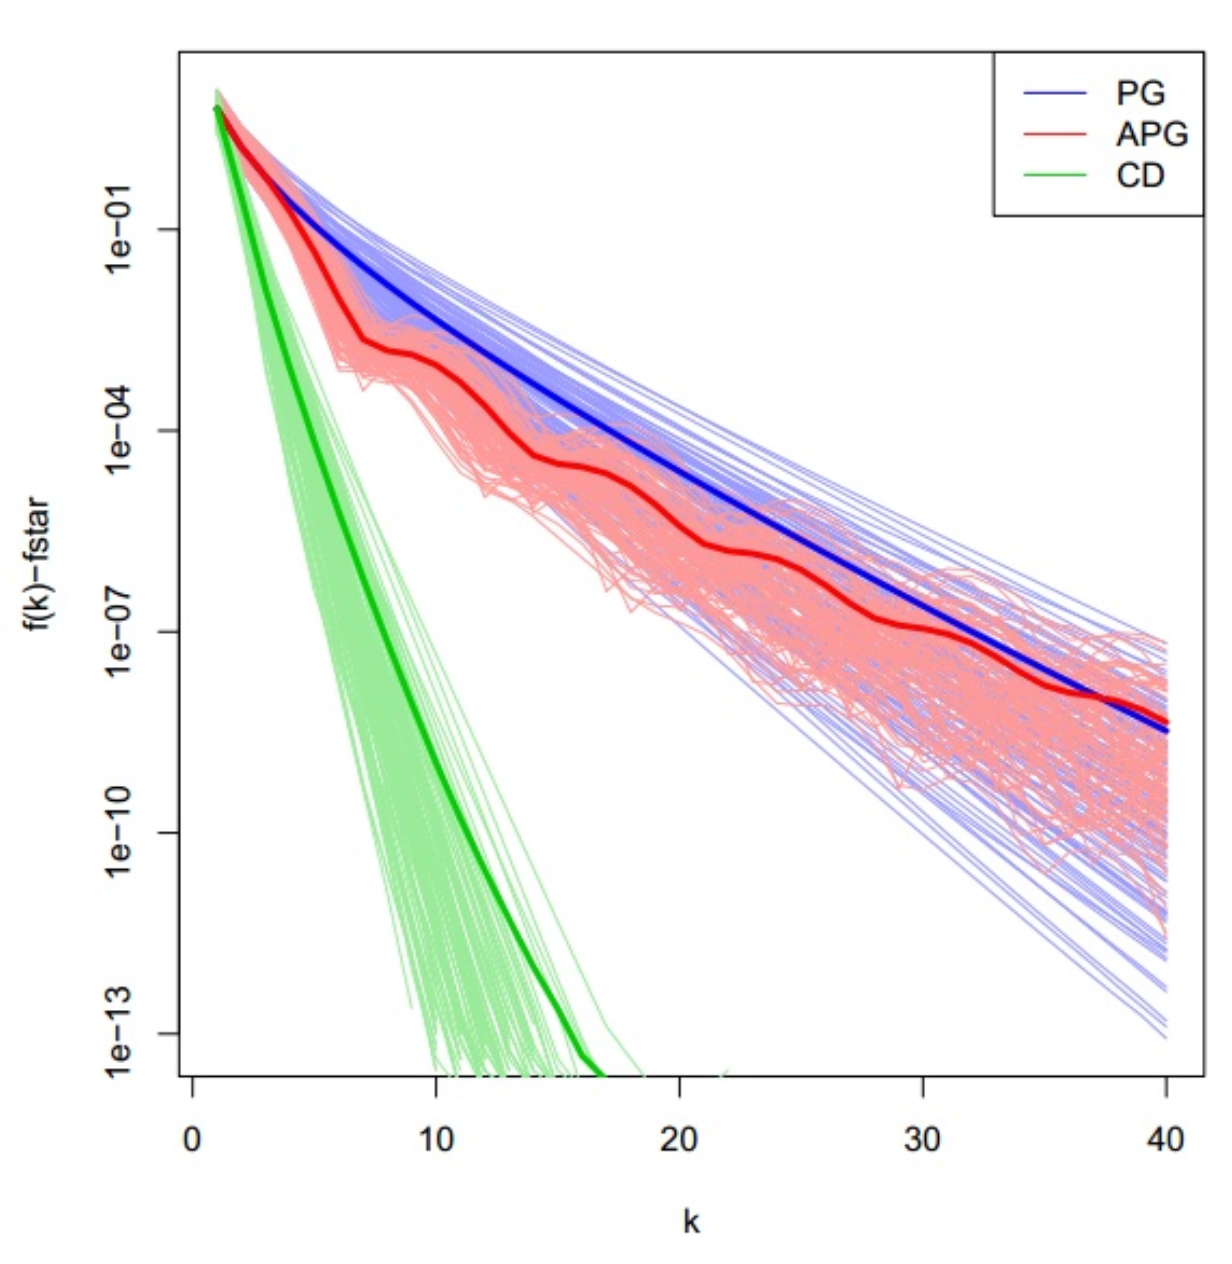
\includegraphics[width=0.5\textwidth]{img/cd_lasso.png}
    \end{center}
    \caption{Coordinate descent and (accelerated) proximal gradient descent for lasso regression with $n=100,p=20$. Note that both GD and CD cost $O(np)$ operators in one cycle.}\label{fig:cd_lasso}
\end{figure}
% The coordinate gradient descent here is comparable to gradient descent for they both share $O(n p)$ flops in each iteration.
\end{frame}

\begin{frame}
    \frametitle{LARS VS Coordinate Descent: Computational Time}
\begin{figure}[!htbp]
    \begin{subfigure}[t]{0.49\textwidth}
        \centering
%		 include first image
        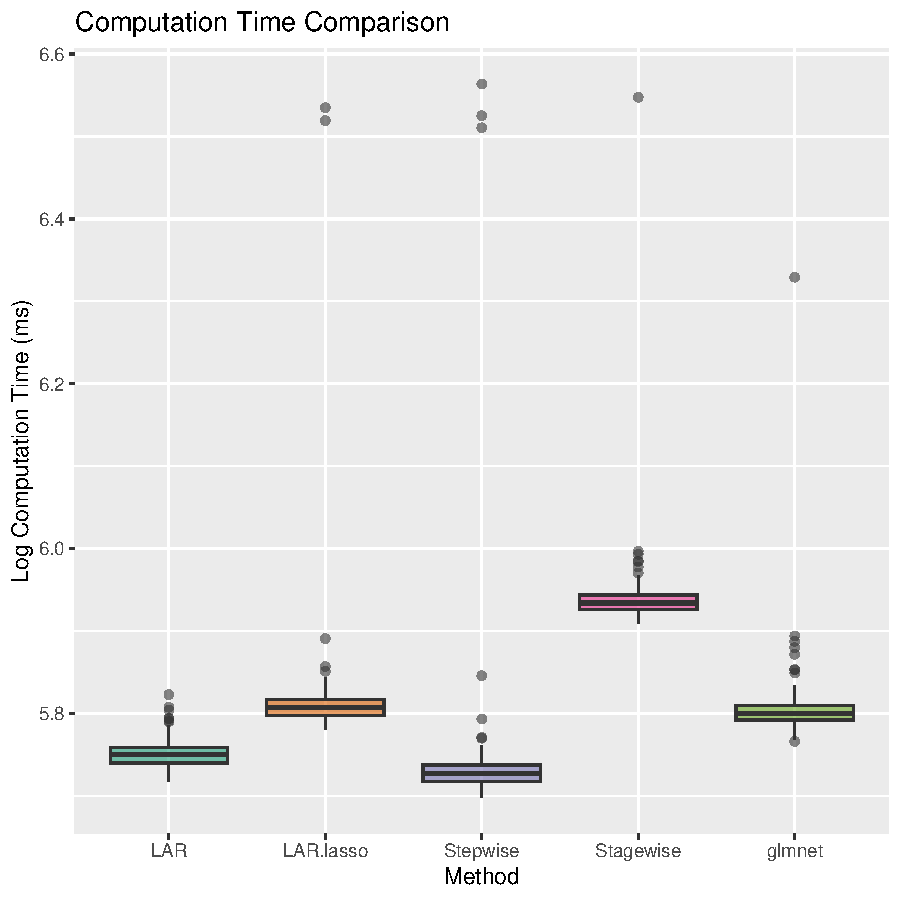
\includegraphics[width=\linewidth]{img/lars_glmnet_time.pdf}
    \end{subfigure}
    \begin{subfigure}[t]{0.49\textwidth}
        \centering
%		 include second image
        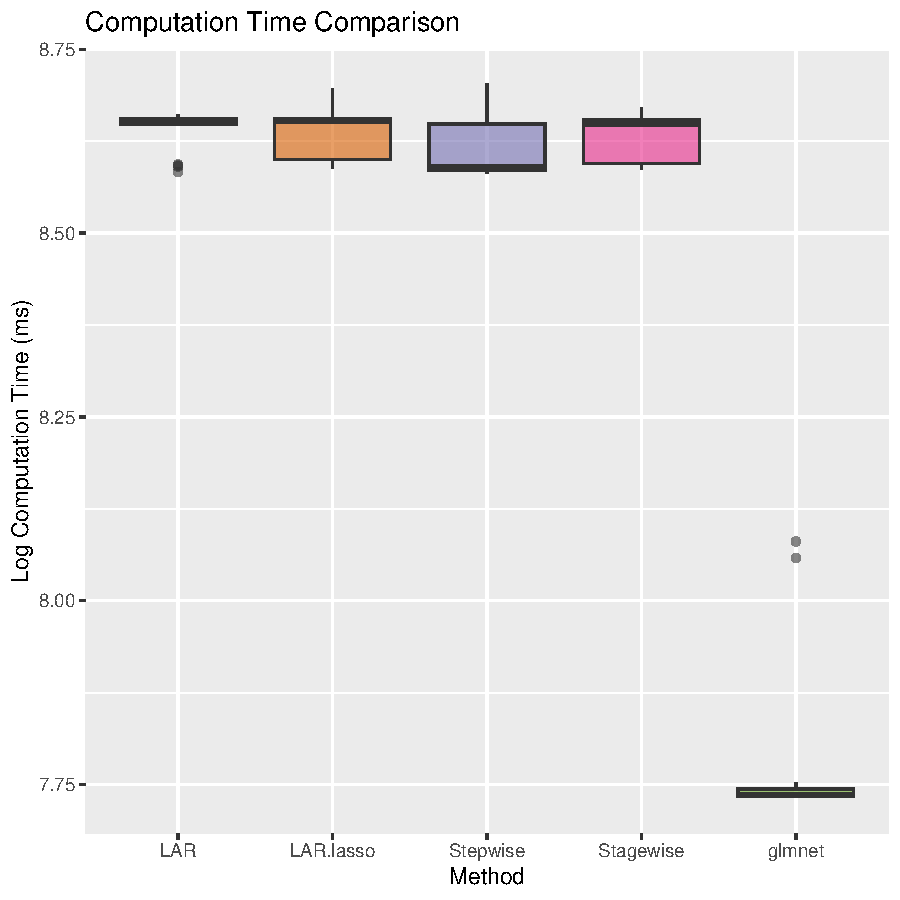
\includegraphics[width=\linewidth]{img/lars_glmnet_time_large.pdf}
    \end{subfigure}
    \caption{Comparison of computational time between LAR, LAR-Lasso, Forward Stagewise Selection, Forward Stepwise Selection and glmnet.lasso with the diabetes data set ($n=442,p=10$) and a simulated data set ($n=1e4,p=200$).}
\end{figure}

\end{frame}